\section{React} 

\subsection{Overview}
React\glosp is a JavaScript library, based on \texttt{npm} and made by Facebook, for building user interfaces by assembling user-defined components.
\subsection{Components}
Components are the core of this \texttt{npm} module. \textit{Soldino} is made of two types of component:
\begin{itemize}
	\item Presentational components;
	\item Container components.
\end{itemize}
\subsubsection{Presentational}
Each presentational component implements \texttt{Component} interface provided by the library. According to this interface, some methods are inherited from the presentational components: in particular our components uses \texttt{Render()} method to render themselves.
Most components can be customized with different parameters when they are created. These creation parameters are called \texttt{props}. Each presentational component returns a single HTML tag, here we can customize the returned tag with some Bootstrap classes. The props are accessible by the components that own them, referencing them with \texttt{this.props.propsName}.

\subsubsection{Containers} 
This type of component is like a wrapper of presentational components. A function called \texttt{Connect(arg1, arg2)} is needed for connecting a container component to a presentational component: in this way we can map some actions and some application state variables inside the presentational component, passing them through props. The \texttt{arg1} is a function called \texttt{mapStateToProps()} and the \texttt{arg2} is another function called \texttt{mapDispatchToProps()}.
\subsection{React-Router} 
React-router-dom is a \texttt{npm} module used for rendering different pages without reloading the entire website, this module works with \texttt{Render()} method provided by each presentational component. \textit{Soldino} is a single page application, so the router, implemented into a JavaScript file called \texttt{App.js}, is responsible to manage which components should be rendered.
\subsection{How to extend with new React component}
To implement a new component with react you have to:
\begin{itemize}
	\item create a new .js file inside \texttt{components/presentational/} and rename it with component's name;
	\item define the render method that returns the GUI of the component, you can use HTML tags or other react components;
	\item you can create its container inside \texttt{components/containers/} and map some props to the component (cf. §6.8);
	\item if you have created a new container you can put it, wherever you want to display it, otherwise you can put the new component;
	\item if you define the new component with some \texttt{args} (e.g. \texttt{<newComponent args="..." />}) you can access to them from component with \texttt{this.props.args}.
\end{itemize}

\subsection{UML} 
\begin{figure}[H]
	\centering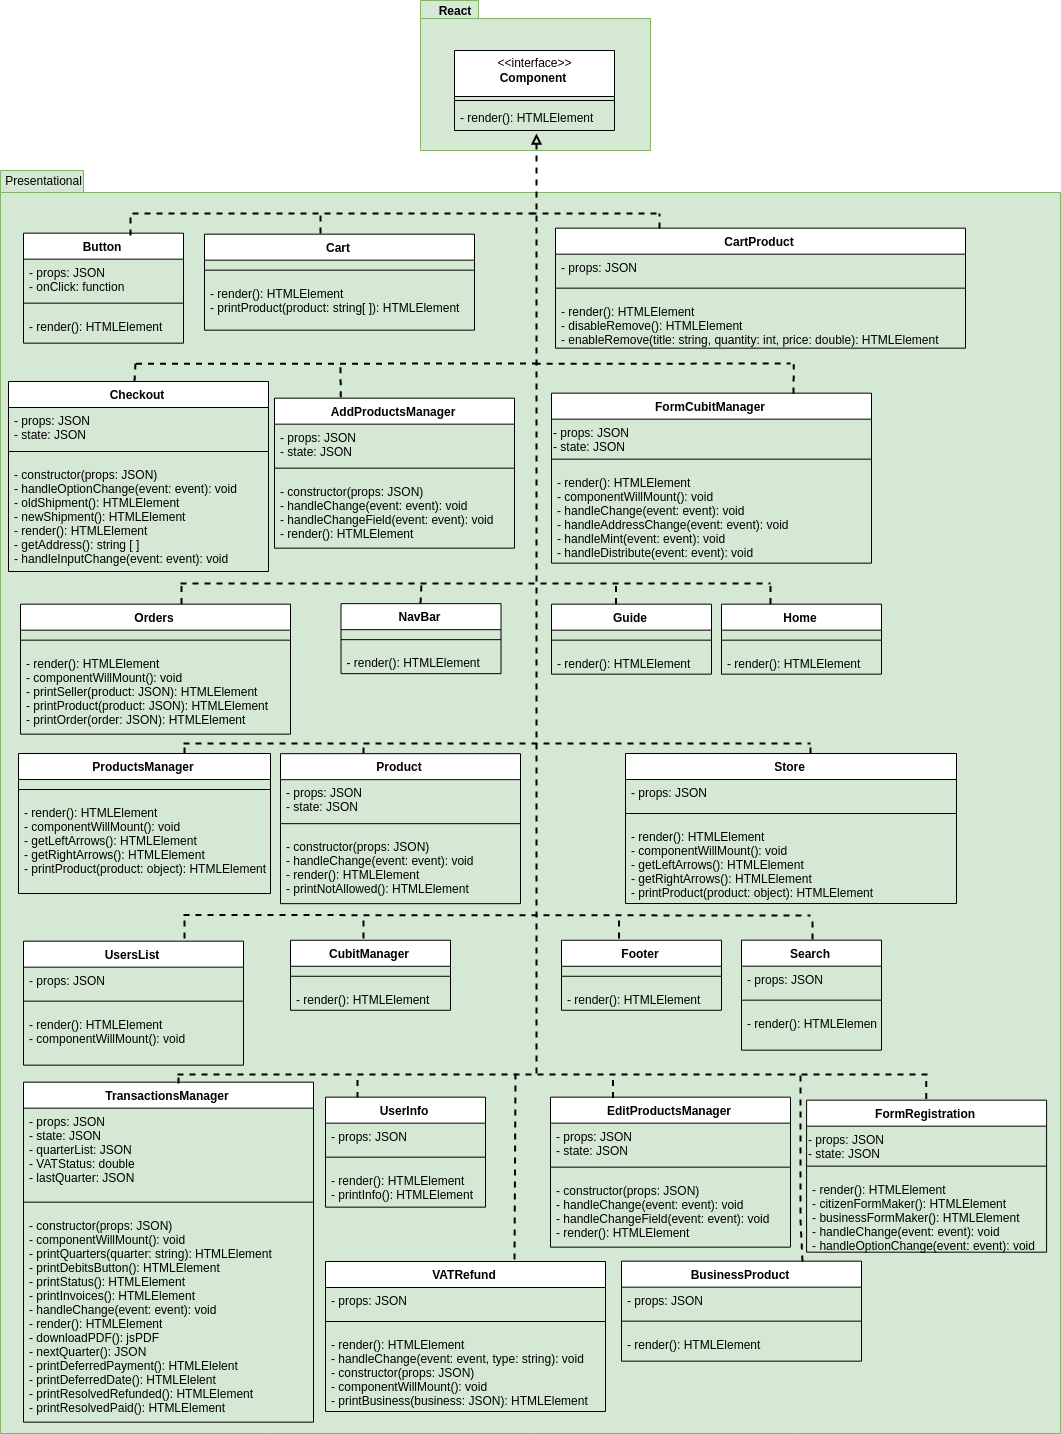
\includegraphics[scale = 0.38]{res/images/Presentational.png}
	\caption{Presentational components}
\end{figure}
\begin{figure}[H]
	\centering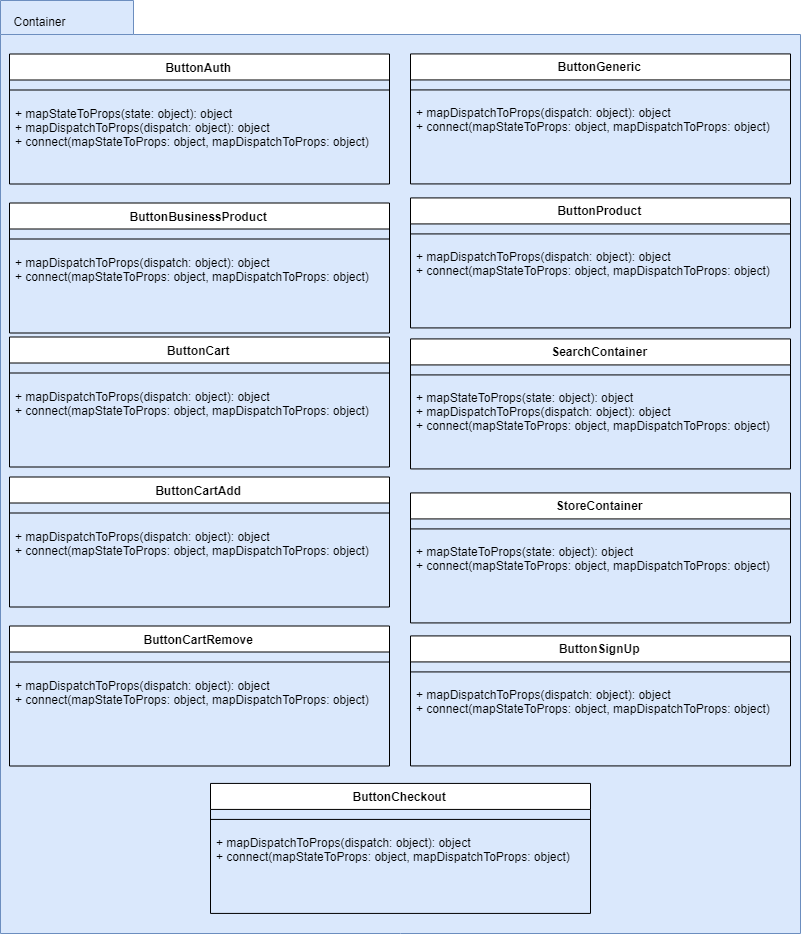
\includegraphics[scale = 0.5]{res/images/Container.png}
	\caption{Container components}
\end{figure}
% \subsection{Collaborations % } if there is one, sequence diag
% \subsection{How to extend} Super optional
